\documentclass[]{article}
\usepackage{graphicx}
\usepackage{float}

%opening
\title{Group 2 - Solar Energy Calculator\\Design description}
\author{  Lukas Hamacek, Aliya Hussain, Charlie H{\"o}glund 
		\\Jonathan Larsson, Sebastian Lindgren, Avalika Podduturu Reddy}

\begin{document}

\maketitle
\pagebreak
\tableofcontents
\listoffigures
\pagebreak

\section{System overview}
\subsection{Background}
The interest for solar energy plants (i.e. photovoltaic plants) has been increasing
a lot during the last years, but the general knowledge about them is still quite
low. However, our client and his colleagues have developed detailed models for
analyzing investment decisions in photovoltaic plants in Sweden. Now, our task
is to develop a user-friendly web-calculator that is based on these models, which
should help to determine what investments in solar energy that are most suitable
for the potential investors. These potential investors are for example private persons and companies. See the project description document for more details.

\subsection{Existing calculators}
There are several already existing solar energy calculators, but most of the current ones are not very user-friendly. A majority of them are also in the form of excel sheets or websites that are not up to date in regard to for example energy-certifications and laws. Here are a few links to some available web-calculators that were given to us by the client:

\begin{itemize}
	\item http://www.elforsk.se/calculator/
	\item http://www.solelprogrammet.se/projekteringsverktyg/berakningsverktyg/
	\item http://www.solkollen.nu/sv\_SE/
	\item http://www.nrel.gov/analysis/tech\_lcoe.html
	\item http://www.energy101.com/free-educational-tools/calculators/
	\item http://re.jrc.ec.europa.eu/pvgis/apps4/pvest.php
\end{itemize}

\subsection{Current system}
The system that is currently being used is in the form of an Excel file (i.e.
one each for private persons and other users), in which the user has to in-
put the necessary default values inside cells and then some built-in functions
calculate the result. Here is a link to the available Excel files on MDH:s website:
http://www.mdh.se/forskning/inriktningar/framtidens-energi/investeringskalkyl-
for-solceller-1.88119
\subsection{Our system}
Our own web application will at least use the same functionalities as the ones
in this already existing system, but bring it to the web. In other words, the
already existing system will not be extended, but instead give us knowledge
about the functional basis on which our web application will be built upon. 

\subsection{Main goals}
The main goals of the calculator is for it to be user-friendly and also easily maintained
by the administrator. Additionally, it should be able to provide both correct and
easily understood results in the form of numerical values, tables and charts. How we will reach these goals and design the system, will be explained in detail in the rest of this document.

\section{Description of the system}
The idea is that you can either use the web-calculator as a registered or non-
registered user. The only difference is that a registered user should be able
to both save calculated results and compare two different calculated results. To calculate the solar energy costs the users should first decide, if they are a private person or other user (e.g. company or property owner), which will determine some of the default input values regarding for example how much taxes to pay. Then the users should 
enter all of the default input values that are necessary for the calculations. In
addition to this, the users also get the opportunity to add extended/advanced
input values, which are meant for the more experienced users, but is not a necessity. When all of the inputs have been
entered, the users should get the calculated results of production cost,
profitability and cash flow in the form of graphical tables and charts.
At the end, the users should also be given the opportunity to download a report file
containing both the input values and the results. Finally, there should be an
administrator (i.e. a registered user) that also can upload an Excel file to update
the input parameters (i.e. the default input values, minimum and maximum
values, and guiding texts). The admin should also be able to download the previously uploaded Excel file just in case. 
\\\\
The desired functionalities of the system have been captured in a use case
diagram which we have created in Figure 1. Besides this there is also a need
for a user-friendly graphical user interface (e.g. through default input values
and guiding texts), to make it easier for the users to navigate and use the web-
calculator.

\begin{figure}[H]
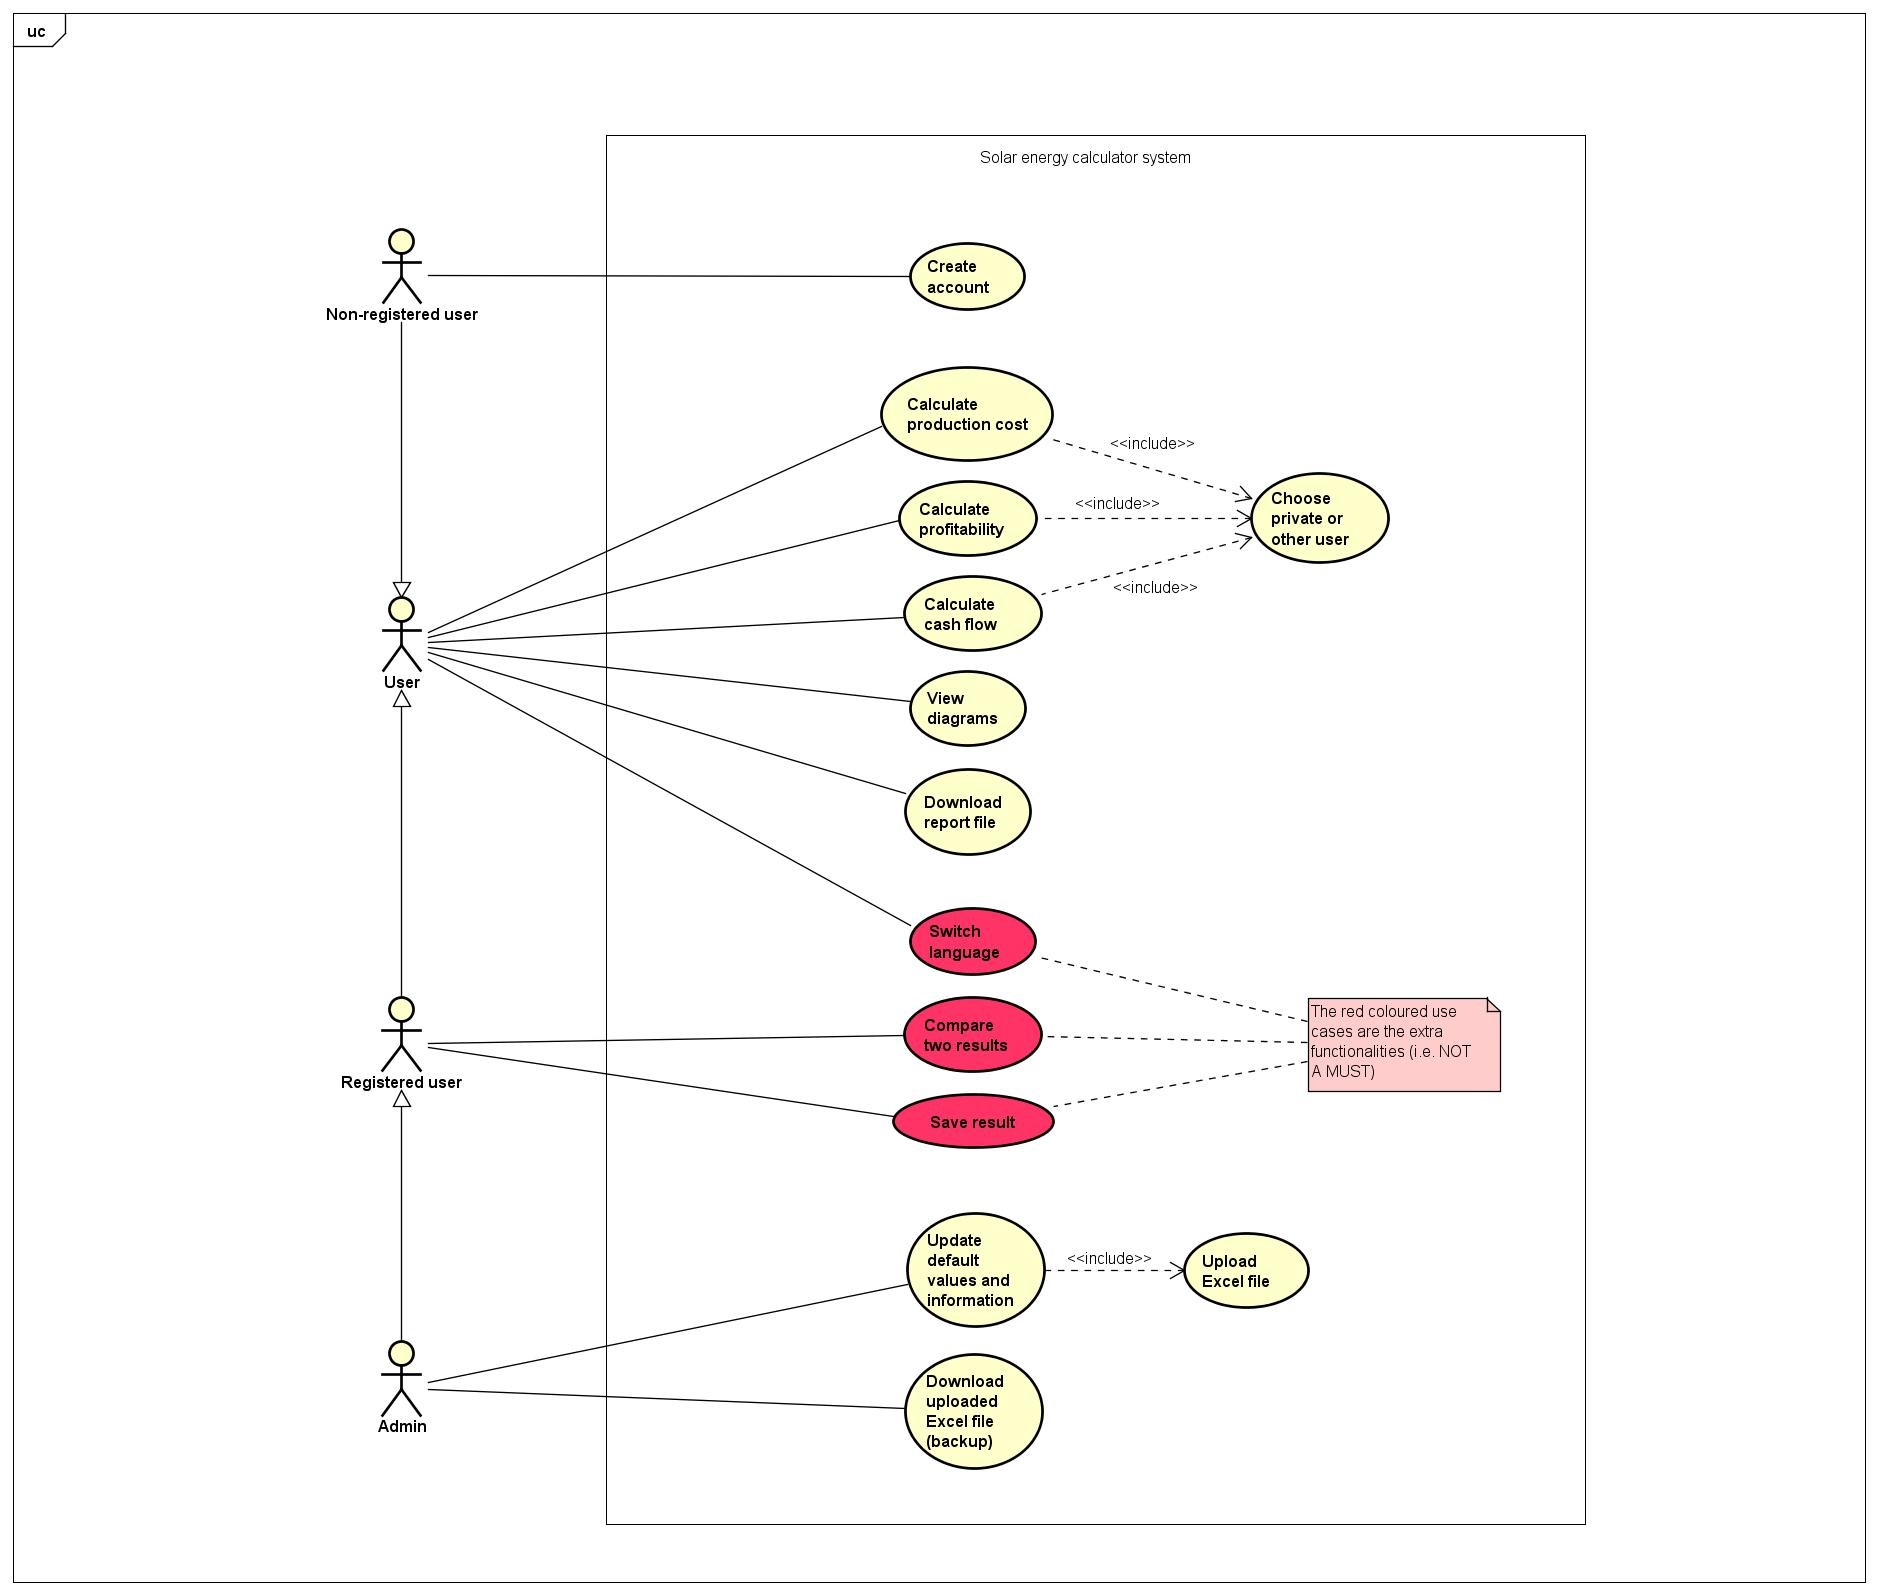
\includegraphics[width=1.0\linewidth]{pic1}
\caption{The use case diagram}
\medskip
\small
The use case diagram covering the desired system functionalities. 
\label{fig:pic1}
\end{figure}


\subsection{Summarized}
The functionality included in the calculator can be summarized as:\\
\textbf{User:}
\begin{enumerate}
	\item Calculate production cost for the PV installations
	\item Calculate profitability for the PV installations
	\item Calculate cash-flow for the PV installations
	\item Output diagrams and get a printable report file
	\item Choose if you are a private person or company
	\item Create account
\end{enumerate}
\textbf{Administrators} can additionally upload a file to update the values on the site and the guiding texts. The administrator will also be able to download a backup file of the previous excel file.

\begin{figure}[H]
	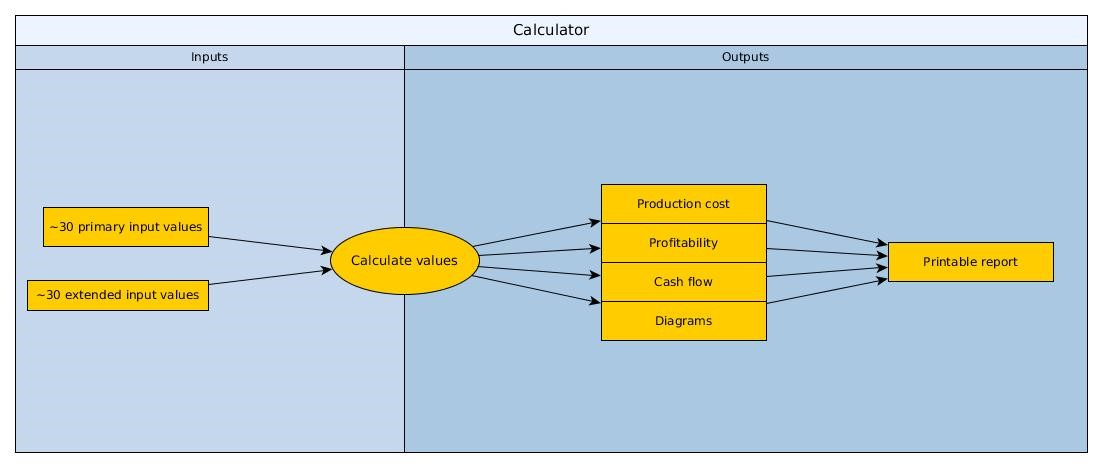
\includegraphics[width=1.0\linewidth]{Bild1}
	\caption{Basic functionality}
	\medskip
	\small
	The basic functionality that we aim to provide the user can be seen here.
	\label{fig:Bild1}
\end{figure}

\subsection{Extra functionality}
Furthermore, the extra desired functionalities of the system have been ranked after importance by the client (i.e. where 1 is the highest and 3 is the lowest). These functionalities are not a must but nevertheless would be appreciated by the client: 

\begin{enumerate}
	\item Compare the calculated values for two sets of input parameters
	\item Save the used input values from one session to another session at a later time
	\item Switch between Swedish and English language
\end{enumerate}

\section{Software architecture}
Here we will talk about the software architecture and other related structure which the website will be built upon. Most important is that we right now aim for using a three-tier architecture for the client-server communication, which makes it easier to make changes to the different parts (i.e. the client, web and database server). 

\begin{figure}[H]
	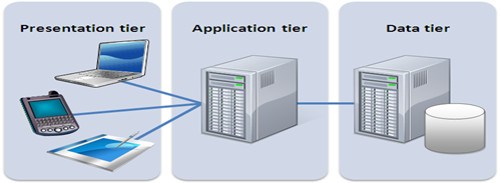
\includegraphics[width=1.0\linewidth]{Bild3}
	\caption{Three tier architecture}
	\medskip
	\small
	We use three tier architecture to be able to build a reliant system which can be scaled in the future if necessary. It also works well for the functionality that the system is supposed to provide. The three tier system is well proved by countless of other applications using it as a foundation.
	\label{fig:Bild3}
\end{figure}

\section{Detailed Software design}
The typical workflow between components is that we have a controller (index.js), api:s (in the api folder) and a view (index.php). The controller will get the information needed from the api and set values in the scope so that the view can use these. 

\subsection{Database}
We will use a MySQL database (link: https://www.phpmyadmin.net/) where
we store login data for the users, the default input parameters to be used (i.e.
based on the latest upload by the admin) and the output report file.

\begin{figure}[H]
	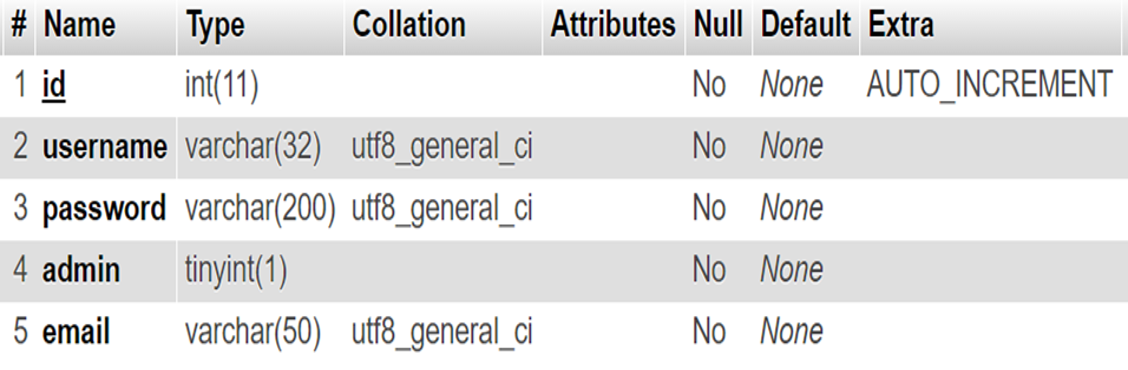
\includegraphics[width=1.0\linewidth]{Bild8}
	\caption{User table}
	\medskip
	\small
	Our user-table is intended for storing multiple users but for the moment it's only used by admin. This might change in the future and the underlying table and basic functionality for login etc. works.
	\label{fig:Bild8}
\end{figure}

\begin{figure}[H]
	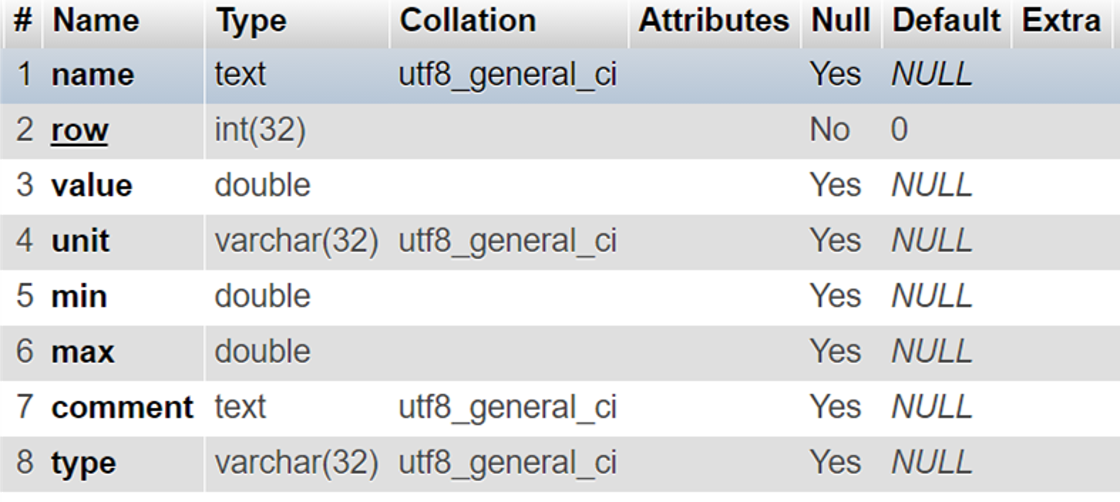
\includegraphics[width=1.0\linewidth]{Bild9}
	\caption{Content table}
	\medskip
	\small
	This table is used for the content in the calculator. The different rows of data that the user has to input and gets a result from is stored here. This is so that the 
	\label{fig:Bild9}
\end{figure}

\subsection{Scripts}
Since our website is a single page application except for the extra page that the
logged in users and admins have (i.e. for the saved results, comparing results,
uploading an excel file), then we will mostly use one large index file (index.php) where all of the HTML is being done. But the PHP and javascript code are probably going to be done in separate files and folders (i.e. to divide the work more evenly). The calculations will be done in JQuery since all of the calculations are static. For the design we will use Bootstrap, which will allow us to use already pre-made buttons, tables, a grid system and other helpful CSS classes. 

\subsection{Extra libraries}
We will use the PHPExcel library for updating the databases default param-
eters through an Excel file, and the Google Charts javascript library for dis-
playing the different output charts. Furthermore, we will also use Meedo (link:
http://medoo.in) for the database handling in order to make the development
faster and more secure, since this comes with help for preventing any type of
SQL injection. Lastly, we will also use the FPDF library for creating the output report files as PDFs.

\section{Graphical User Interface}
Most of the functionality is described in previous sections. Here you'll instead get a taste of how the GUI is looking at the moment.

This website is not complete, it is missing the following things: A separate admin page (i.e. for uploading and downloading excel files), a separate page for saved and compared results for registered users... But these will be added in due time and follow the same graphical model.

Right now we don't have the calculations either but they will be there later. Soon there will be diagrams, tables etc. as well.

\begin{figure}[H]
	
\includegraphics[width=1.0\linewidth]{pic2}
	\caption{The header of the start page}
	\medskip
	\small
	Here you can see a navigation bar with the buttons for going to the calculator (i.e. “start now” button included), about and contact section of the start page. You can also see the sign in button for the registered users.
	\label{fig:pic2}
\end{figure}
\begin{figure}[H]
	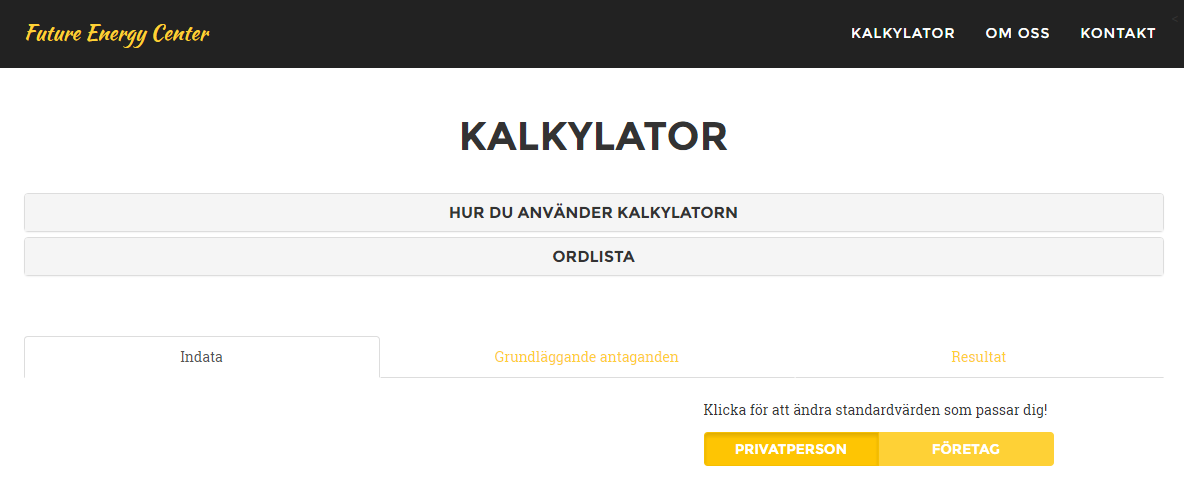
\includegraphics[width=1.0\linewidth]{pic3}
	\caption{The calculator section}
	\medskip
	\small
	Here you can see the calculator section of the start page. Here you can learn more about the words you might need to know and how to use the calculator. This improves the users' understanding of the system.
	\label{fig:pic3}
\end{figure}

\begin{figure}[H]
	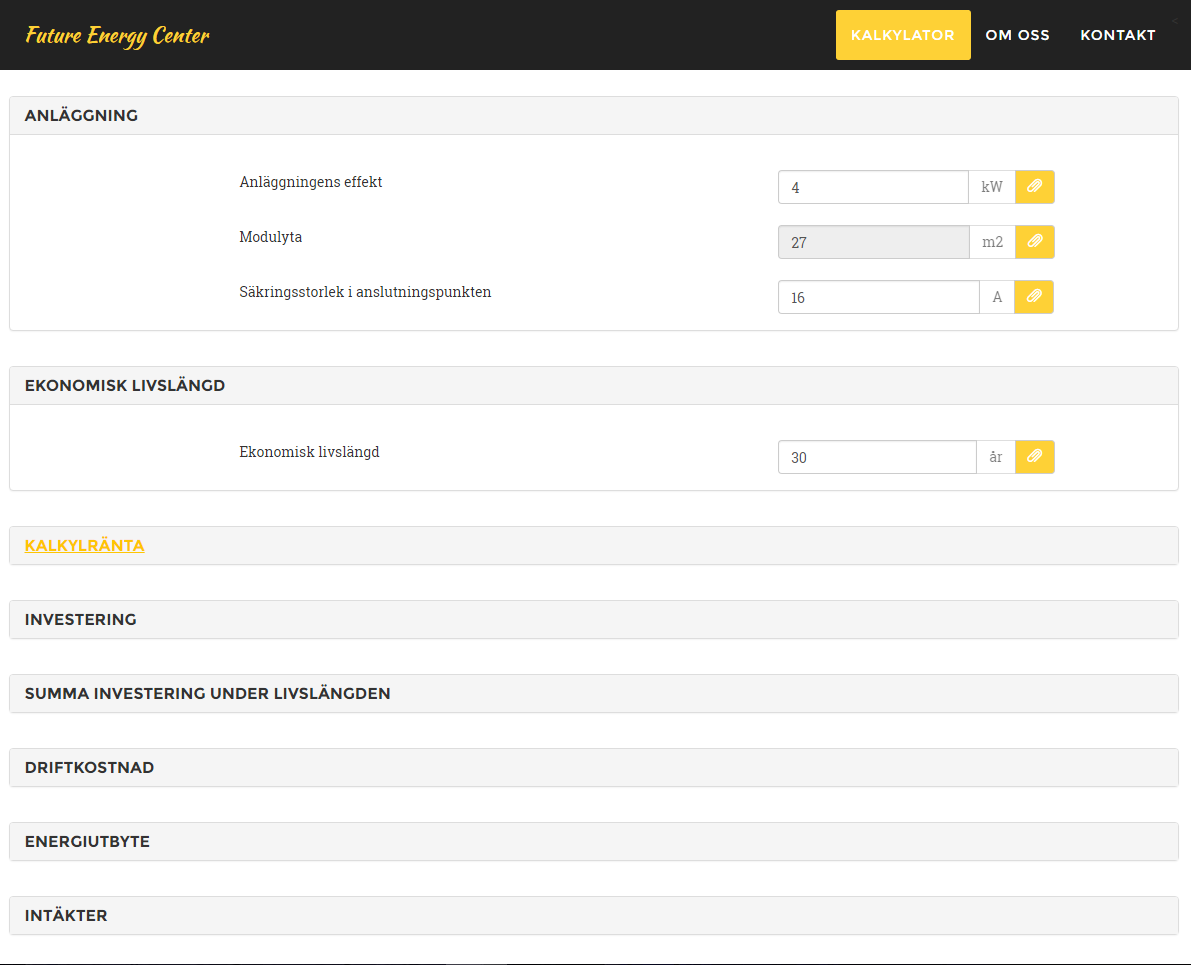
\includegraphics[width=1.0\linewidth]{Bild7}
	\caption{The calculator section}
	\medskip
	\small
	When you enter values you can enter then to the fields indata or grundläggande antaganden. These stand for the basic and extended values. When clicking one of the sections you will see underlying data columns. You then click on and fill the values that you need. The result will later be displayed under the results button.
	
	Also notice the “person” and “company” buttons where the users can decide what kind of customer they are. 
	\label{fig:Bild7}
\end{figure}

\begin{figure}[H]
	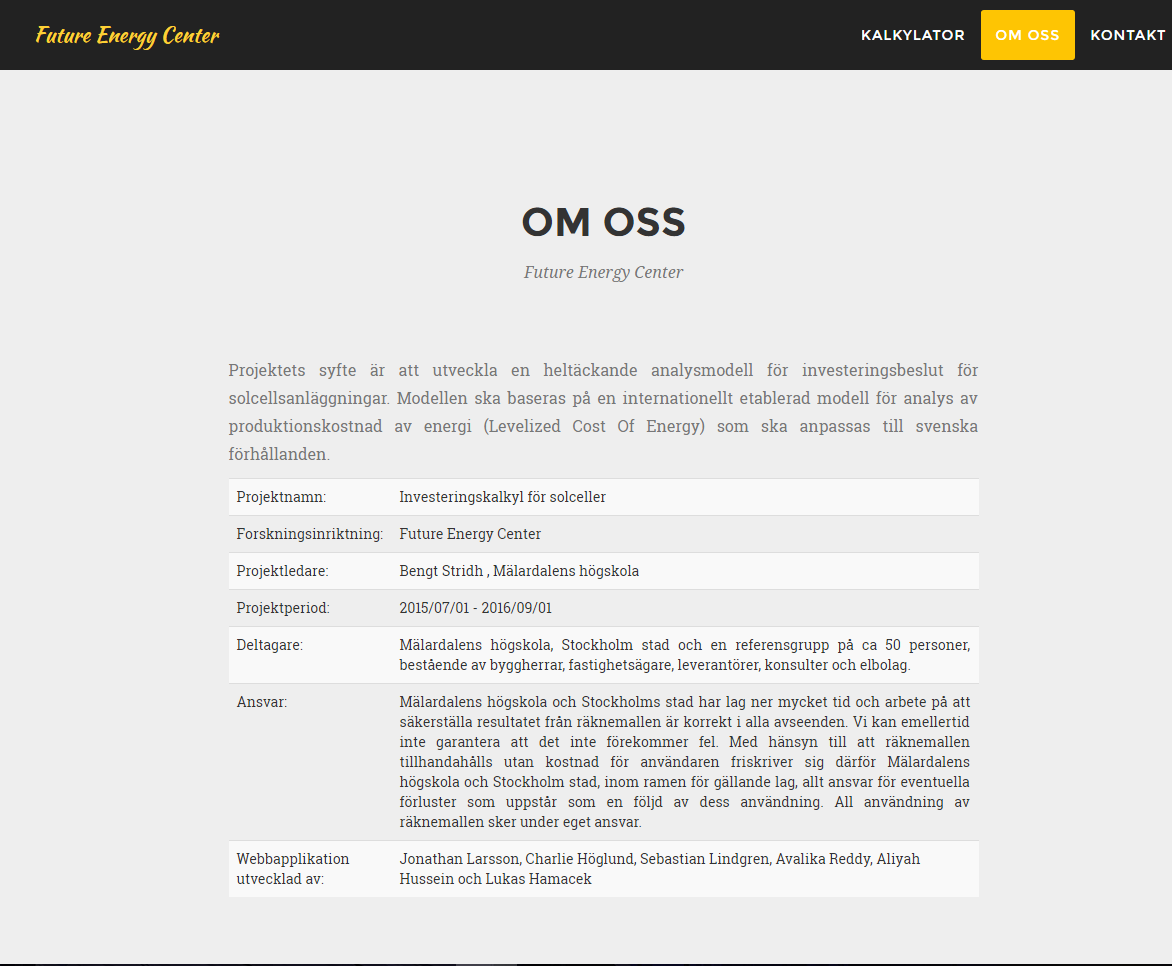
\includegraphics[width=1.0\linewidth]{pic4}
	\caption{The about section}
	\medskip
	\small
	Here you can see the about section of the start page. It simply contains information about the researchers and their project, which will be updated later on. 
	\label{fig:pic4}
\end{figure}
\begin{figure}[H]
	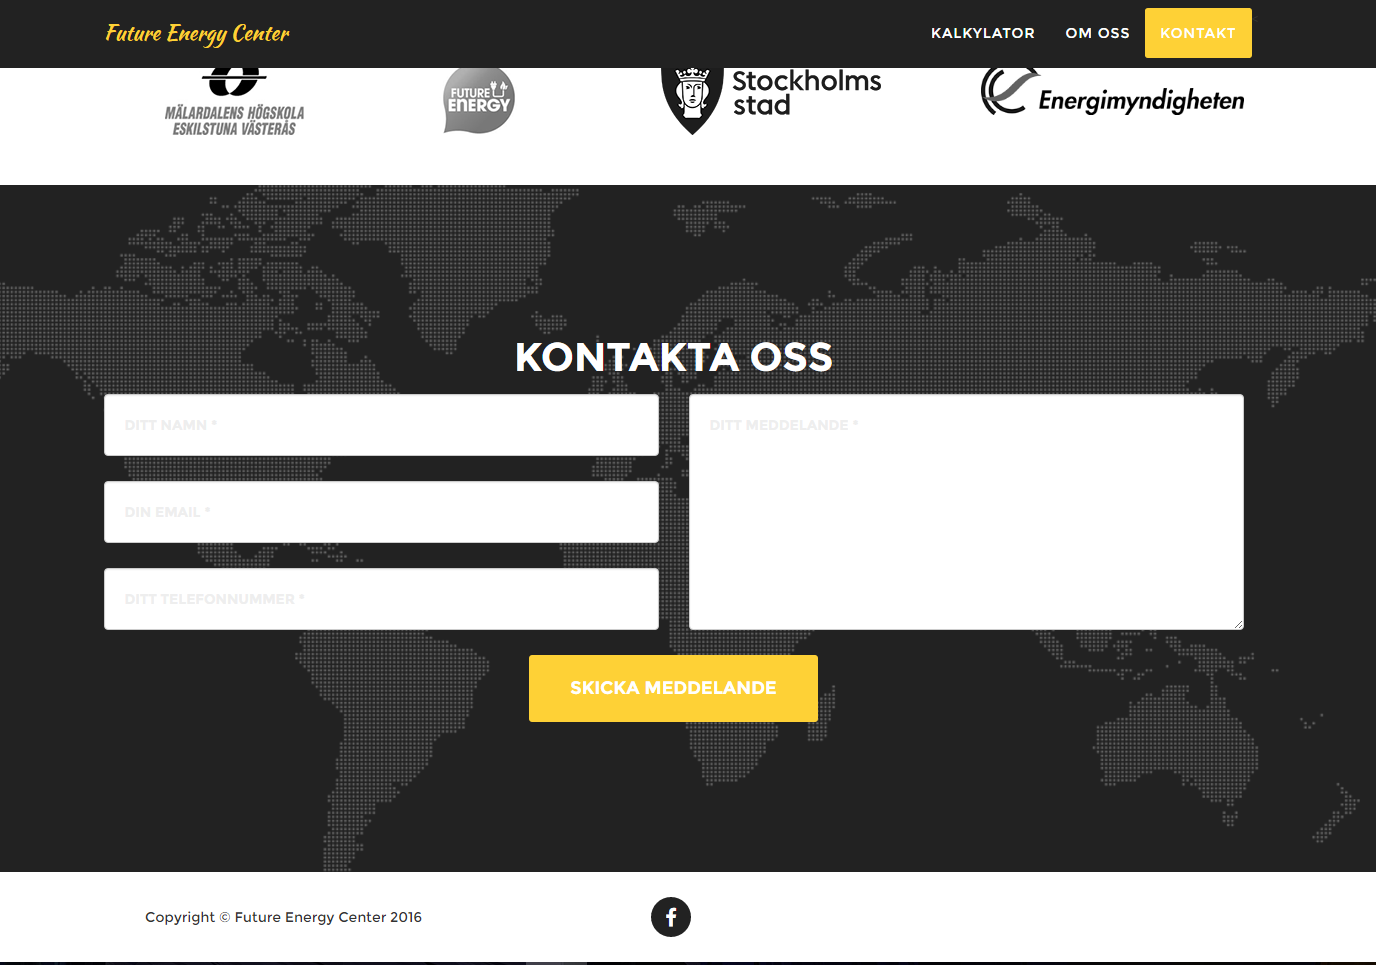
\includegraphics[width=1.0\linewidth]{pic5}
	\caption{The contact section}
	\medskip
	\small
	Here you can see the contact section of the start page. It simply contains input boxes and a button for contacting the owners of the website.
	\label{fig:pic5}
\end{figure}
\begin{figure}[H]
	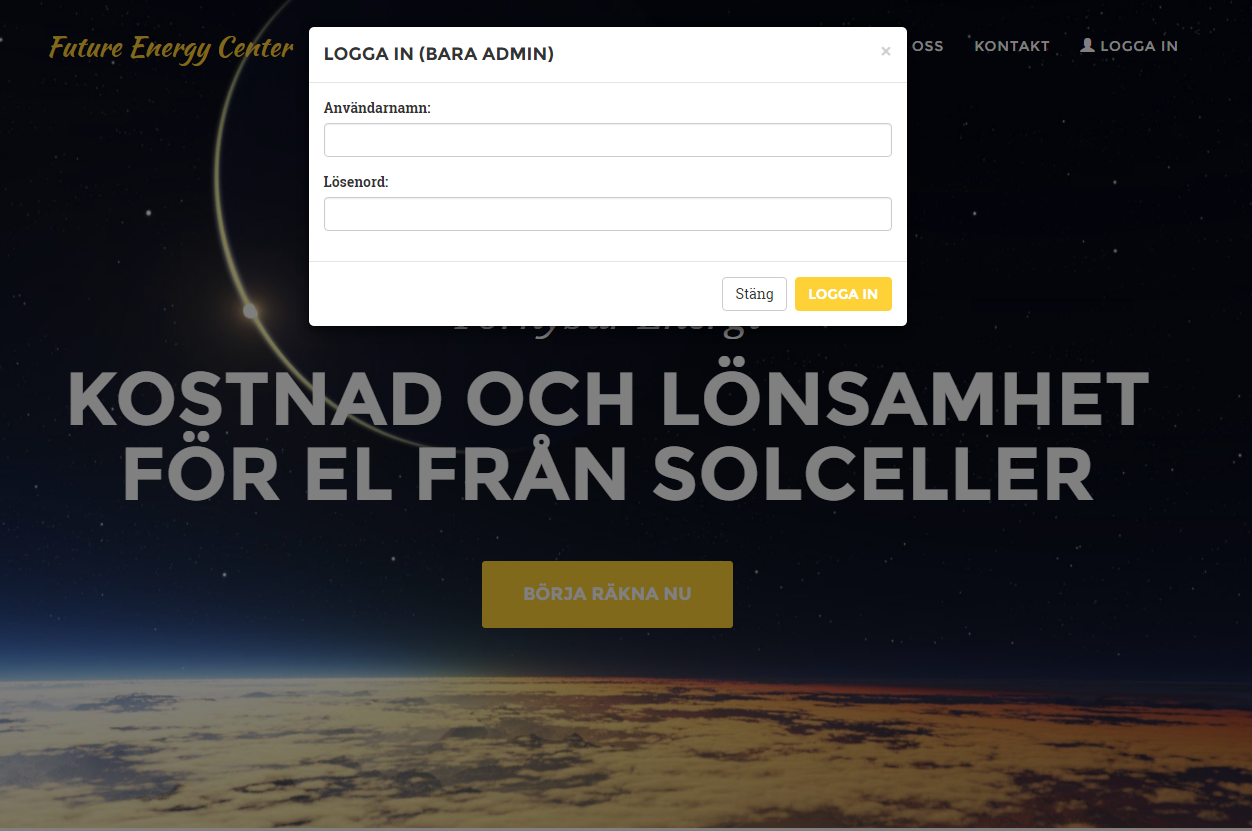
\includegraphics[width=1.0\linewidth]{pic6}
	\caption{Login modal}
	\medskip
	\small
	Here you can see the hidden login window which you can access manually if you are the admin.
	\label{fig:pic6}
\end{figure}
\begin{figure}[H]
	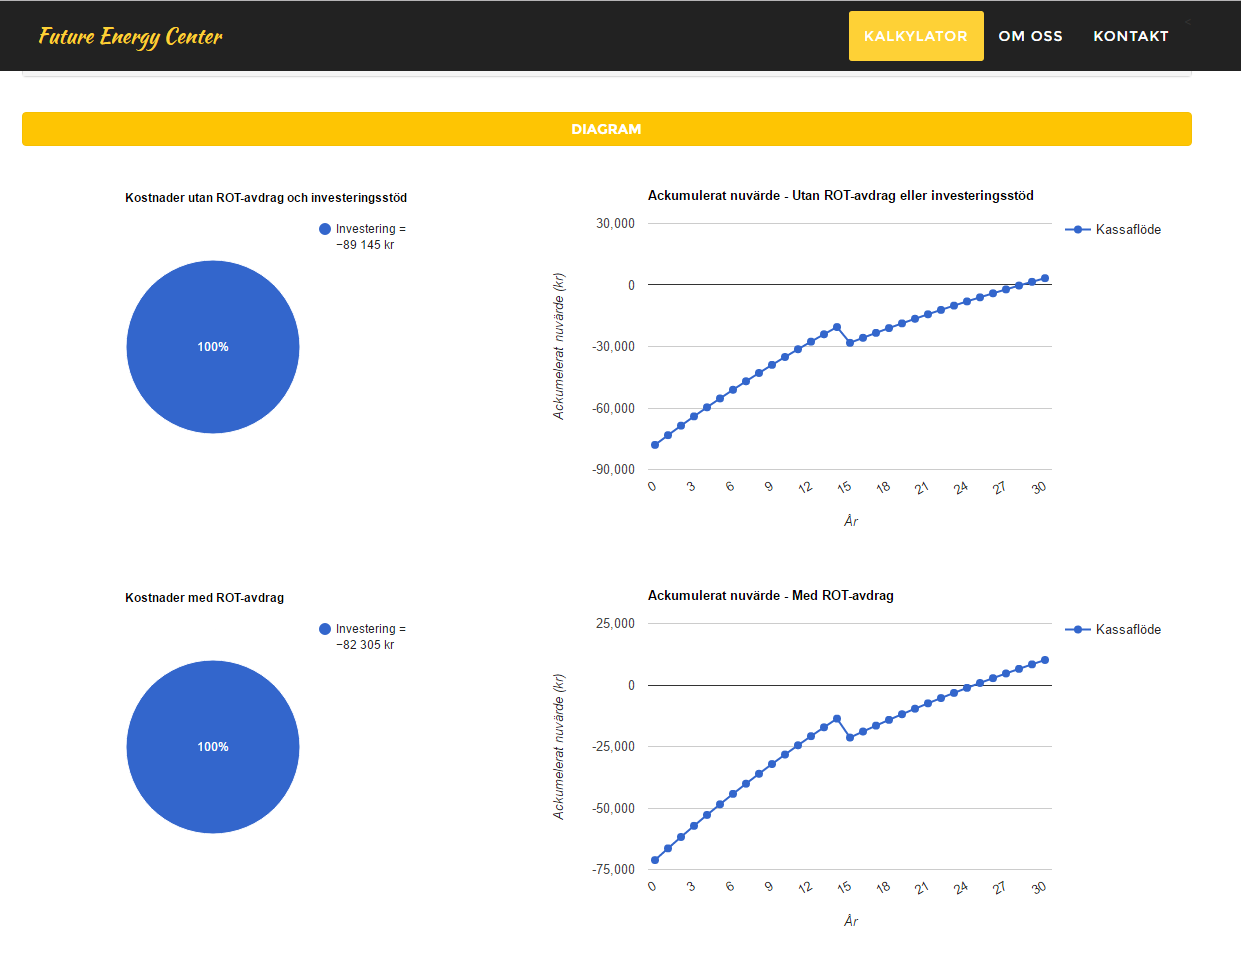
\includegraphics[width=1.0\linewidth]{pic7}
	\caption{Pie sharts for better overview of calculations}
	\medskip
	\small
	Here you can see the pie charts that show the result of the calculations.
	\label{fig:pic7}
\end{figure}

\begin{figure}[H]
	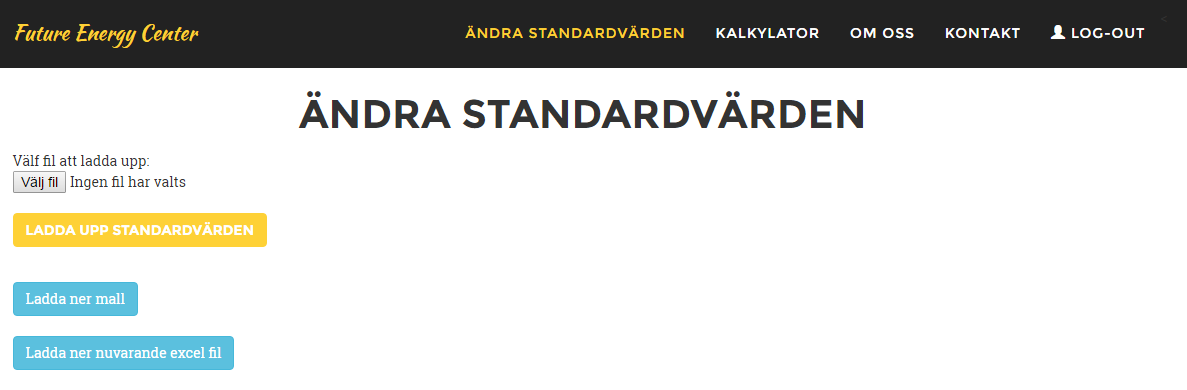
\includegraphics[width=1.0\linewidth]{pic8}
	\caption{Uploading excel files to update}
	\medskip
	\small
	Here you see the uploading of an excel file functionality, and downloading the backup excel file (I.e. this is only the admin but could be extended to other users in the future).
	\label{fig:pic8}
\end{figure}

\end{document}